\documentclass{standalone}
\usepackage{tikz}
\usepackage{rotating}

\usetikzlibrary{angles}

\begin{document}
	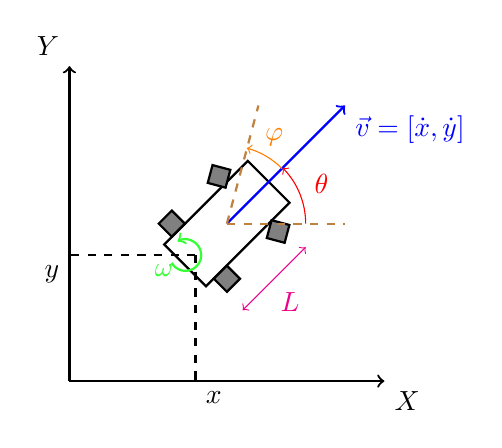
\begin{tikzpicture}
		\draw[thick,->] (0,0) -- (4,0) node[anchor=north west] {$X$};
		\draw[thick,->] (0,0) -- (0, 4) node[anchor=south east] {$Y$};
		\node(ROBOT) at (2, 2)[rectangle, draw, thick, minimum width=1.5cm, minimum height=0.75cm, rotate=45]{};
		\node(L1) at (1.9, 2.6)[rectangle, draw, thick, minimum width=0.1cm, minimum height=0.1cm, fill=gray, rotate=75]{};
		\node(L2) at (2.65, 1.9)[rectangle, draw, thick, minimum width=0.1cm, minimum height=0.1cm, fill=gray, rotate=75]{};
		\node(L3) at (1.3, 2)[rectangle, draw, thick, minimum width=0.1cm, minimum height=0.1cm, fill=gray, rotate=45]{};
		\node(L4) at (2, 1.3)[rectangle, draw, thick, minimum width=0.1cm, minimum height=0.1cm, fill=gray, rotate=45]{};
		\draw[blue, thick,->] (2, 2) -- (3.5, 3.5) node[blue, anchor=north west] {$\vec{v}=[\dot{x}, \dot{y}]$};
		\draw[thick,dashed] (1.6, 1.6)--(1.6, 0) node[anchor=north west] {$x$};
		\draw[thick,dashed] (1.6, 1.6)--(0, 1.6) node[anchor=north east] {$y$};
		\draw[red, ->] (3, 2) arc (0:45:1cm);
		\node[red] at (3.2, 2.5) {$\theta$};
		\draw[green!80, thick, ->] (1.3, 1.5) arc (-150:120:0.2cm);
		\node[green!80] at (1.2, 1.4){$\omega$};
		\draw[magenta, <->] (2.2, 0.9) --(3, 1.7);
		\node[magenta] at (2.8, 1){$L$};
		\draw[thick, dashed, brown] (2, 2) --(2.4, 3.5);
		\draw[thick, dashed, brown] (2, 2) --(3.5, 2);
		\draw[orange, ->] (2.7, 2.7) arc (45:75:1cm);
		\node[orange] at (2.6, 3.1){$\varphi$};
	\end{tikzpicture}
\end{document}